\documentclass[12pt]{report}
%\renewcommand{\chaptername}{Kapitel}
% UTS Thesis style
% Options
%
% 	demo 	Sets graphicx package to demo, 
%			ie does not require the actual images files.
%
%   sans    Font
%
%	roman	Font
%
%	neverindent
%
% 201505

%\usepackage[sans]{uts_thesis}

\usepackage[sans]{uts_thesis}
\usepackage{hyperref}

\usepackage[style=authoryear,backend=bibtex8]{biblatex}
\usepackage[ngerman]{babel}
\usepackage{float}
\usepackage[]{acronym}
\usepackage{hyperref}
\usepackage{subfiles}
\usepackage[german]{algorithm2e}



% use "disable" as argument for the todonotes package 
% to switch of all todos and the todolist in the 
% document. e.g. \usepackage[disable]{todonotes} 
\usepackage[disable]{todonotes} 




\addbibresource{./references.bib}
\graphicspath{ {images/} }

%\includeonly{abstract,introduction}

\begin{document}
% note using \include in main.tex instead of \input because of 
%	1) .aux file caching 
%	2) \includeonly
% \include is equivalent to \input() \clearpage, 
%	so it might not be appropriate inside chapters, use \input
% TODO UTS FEIT Dissertations usually have a subtitle
\title{
	{Seminararbeit Führungstraining}\\
	{\large eingereicht in der Modulbibliothek - Führungstraining im WS2015}\\
	{\large bei}\\
	{\large Dr. Antje Duden \& Dipl. Betriebswirtin Uschi Pferrer}\\ [1cm]
	{
\includegraphics[scale=0.5]{logo/FHVlogo1.png}} \\ [1cm]
	%{\includegraphics[width=0.25\linewidth]{images/logo/qrcode}}
}
\author{Martin Münch BSc}
\date{01. November 2015}



\maketitle



\tableofcontents

\listoftodos	% http://mirror.easyname.at/ctan/macros/latex/contrib/todonotes/todonotes.pdf

\chapter{Einleitung}
\label{chap:einleitung}

Der Apriori Algorithmus ist ein, im IBM-Almaden-Forschungszentrum entwickeltes, klassisches Verfahren der Assoziationsanalyse. Er findet sinnvolle oder nützliche Zusammenhänge in transaktionsbasierten Datenbanken und bildet diese in Assoziationsregeln ab. Ein häufiger Anwendungsfall wäre die Analyse des Kaufverhaltens von Kund\_innen bzw. die Warenkorbanalyse.
\parencite [s.][S. 109, S.112] {Datawarehouse}


\paragraph{Assoziationsanalyse}
Assoziationsanalyse ist ein Bereich des Data Mining und bezeichnet die Suche nach 'starken' Regeln. Daraus folgen Assoziationsregeln, die Korrelationen zwischen gemeinsam auftretenden Ereignissen beschreiben.

\paragraph{Assoziationsregeln}
Assoziationsregeln beschreiben Korrelationen zwischen zwei Ereignissen (mit einer bestimmten Wahrscheinlichkeit) in der Form $ A \rightarrow B $ .\\
Um solche Zusammenhänge zu erkennen werden Datenbestände bezüglich der Häufigkeit des gleichzeitigen Auftretens von Objekten bzw. Ereignissen untersucht.\parencite [s.][S.110]{Datawarehouse}
Ein Beispiel für solche Zusammenhänge wäre:

Wenn Windeln gekauft werden, wird auch Bier gekauft.

Um die abgeleiteten Assoziationsregeln zu bewerten und Aussagen über diese treffen zu können, werden zwei probabilistische Messwerte herangezogen: Support und Konfidenz.

\paragraph{Support}
Der Support weist auf die Bedeutung von Elementen in einer Menge hin, je höher der Support desto höher die Bedeutung der Elemente.
\parencite [s.][S.110]{Datawarehouse}

\paragraph{Konfidenz}
Mit der Konfidenz wird die Stärke einer Regel ausgedrückt. Auch bei der Konfidenz ist ein hoher Wert wünschenswert, sie beschreibt salopp formuliert die 'Treffsicherheit' einer Assoziationsregel.
\parencite [s.][S.110]{Datawarehouse}


\chapter{Methode}
Die Datenbasis $D$ ist eine denormalisierte Tabelle, mit einer Menge von Items $I$, die die Spalten der Tabelle darstellen und Transaktionen $\{t_1,t_2,...,t_n\}$, wobei eine Transaktion eine Zeile in der Tabelle ist.
\\
\\
Ein Beispiel für eine Datenbasis sind alle Verkaufstransaktionen innerhalb eines bestimmten Zeitraumes, eine Transaktion ist ein Kund\_inneneinkauf, wobei Items die Artikel im Sortiment sind. 
\parencite[s.][1 Introduction]{IBM}
\\
\\
Wie bereits in der ~\nameref{chap:einleitung} erwähnt werden Assoziationsregeln und Mengen anhand von Support und Konfidenz bewertet.

\section{Support}
Der Support kann einerseits für Mengen von Items berechnet werden, andererseits aber auch für Assoziationsregeln selber.
\subsection{Support einer Menge von Items}
Der Support gibt Auskunft über die Wichtigkeit einer Menge von Items bzw. die Wahrscheinlichkeit mit der die Itemmenge in einer Transaktion vorkommt.
\\
\\
Der Support einer Teilmenge $X=\{A_1, A_2,...,A_n\}$ wird wie folgt berechnet:\\
\begin{equation}
Support(X) = P(A1, A2, ... , An)= \frac{\mid \{t \in D \mid  X \subseteq  t\}\mid}{\mid D \mid}
\end{equation}

Beispiel: 
Der Support der Itemmenge \{Milch\}, ist der Prozentsatz der Kund\_innen die während ihres Einkaufs unter anderem Milch gekauft haben.\parencite[s.][S. 171f]{TU_Dortmund}

\subsection{Support einer Assoziationsregel}
Der Support einer Assoziationsregel $X \rightarrow Y$ ist definiert als der Support von Prämisse/Grundlage($X$) und Konklusion/Folgerung($Y$). Er gibt die relative Häufigkeit an mit der die Regeln in der Datenbasis vorkommt.
Der Support einer Assoziationsregel $X \rightarrow Y$, wobei $X=\{A_1,A_2,...,A_n\}$ und $Y=\{B_1,B_2,...,B_n\}$ wird wie folgt berechnet:\\
\begin{eqnarray}
Support(X \rightarrow Y)= Support(X \cup Y) =  \\
P(A_1, A_2, ... , A_n, B_1, B_2, ..., B_n) = \frac{\mid \{t \in D \mid  X \cup Y \subseteq  t\}\mid}{\mid D \mid}
\end{eqnarray}
\parencite[s.][S. 173]{TU_Dortmund}

\section{Konfidenz}
Die Konfidenz einer Assoziationsregel  $X \rightarrow Y$  wobei  $X=\{A_1,A_2,...,A_n\}$ und $Y=\{B_1,B_2,...,B_n\}$, entspricht der Wahrscheinlichkeit der Konklusion/Folgerung ($Y$) unter Bedingung der Prämisse/Grundlage ($X$). Das bedeutet die Konfidenz einer Assoziationsregel ist der (relative) Anteil der Transaktionen die sowohl X, wie auch Y enthalten. Sie misst sozusagen die Treffsicherheit einer Assoziationsregel.
\\
Die Konfidenz einer Assoziationsregel wird wie folgt berechnet:
\begin{equation}
Confidence(X \rightarrow Y) = Support(X \cup Y)/ Support(X)
\end{equation}
\parencite[s.][S. 173f]{TU_Dortmund}
\newpage

\section{Algorithmus}
Der Apriori Algorithmus arbeitet in zwei Schritten, 1. dem Finden häufiger Mengen, und 2. der Erzeugung von Assoziationsregeln, beide verwenden die Subroutine Apriori Gen.
\\
\\
\begin{algorithm}[H]
\label{alg:apriori}
	\KwIn{$minsupp$, $minconf$}
	\KwOut{Assoziationsregeln}
	1. Schritt: Finden häufiger Mengen\;
	2. Schritt: Erzeugung von Assoziationsregeln\;
\caption{Apriori Algorithmus \parencite[s.][S. 93]{Business_Intelligence}}
\end{algorithm}
\bigskip


\subsection{1. Schritt:  Finden häufiger Mengen}

Die Idee des Apriori Algorithmus (Algorithmus \ref{alg:schritt1}) basiert darauf, dass alle Teilmengen einer häufigen Teilmenge ebenfalls häufig sind, und alle Obermengen einer nicht-häufigen Itemmenge (Teilmenge) ebenfalls nicht häufig sind. 
Das bedeutet, dass Kandidatenmengen mit $k$ Items durch Zusammenführung von Itemmengen mit $k-1$ Items generiert werden könnnen. Alle jene, die Teilmengen, die nicht häufig sind, enthalten werden gelöscht. Häufige Mengen sind nur solche, die genügend hohen Support (mindestens $minsupp$) haben. 
\parencite[s.][2 Discovering Large Itemsets
]{IBM}
\parencite[s.][S. 175]{TU_Dortmund}
\begin{equation}
I_1 \subseteq I_2 \ \mbox{impliziert} \ Support(I2) \leq Support(I_1)
\end{equation}
\bigskip
\bigskip

\begin{algorithm}[H]
\label{alg:schritt1}
	\KwIn{Datenbasis mit Transaktionen, $minsupp$}
	\KwOut{häufige Itemmengen}
	generiere häufige Itemmengen $L_1$ mit $k=1$\;
	\While{solange neue häufigen Mengen gefunden werden}{
		generiere Kandidatenmengen $C_k$ mit ~\nameref{alg:apriorigen} \;
		berechne den Support der Kandidatenmengen\;
		Aufnahme der Mengen mit genügend hohem Support in $L_k$\;
		k++;
	}
	Ausgabe der häufigen Mengen\;	
\caption{Bestimmen häufiger Itemmengen mit Support $\geq minsupp$ \parencite[s.][S. 176]{TU_Dortmund}, \parencite[s.][2.1 Algorithm Apriori]{IBM}}
\end{algorithm}


\subsection{AprioriGen}
AprioriGen (Algorithmus \ref{alg:apriorigen}) ist eine Subroutine des Apriori Algorithmus (Algorithmus \ref{alg:apriori}) und wird sowohl zur Berechnung häufiger Mengen, wie auch zur Erzeugung von Assoziationsregeln verwendet.
\\
Der AprioriGen Algorithmus nutzt aus, dass jede $k-1$ Teilmenge einer Menge aus $L_k$ in $L_{k-1}$ enthalten sein muss. 
\\
\\
\begin{algorithm}[H]
\label{alg:apriorigen}
	\KwIn{Menge häufiger $k-1$ Itemmengen $L_{k-1}$}
	\KwOut{Obermenge $C_k$ der Menge $L_k$}
	1. je zwei häufige $L_{k-1}$ werden mit gleichen ersten ($k-2$) Elementen werden zu einer Kandidatenmenge $C_k$ vereinigt\;
	2. entferne aus $C_k$ diejenigen Itemmengen, deren ($k-1$) Teilmengen nicht alle in $L_{k-1}$ liegen\;
\caption{AprioriGen, \parencite[s.][2.1.1 Apriori Candidate Generation
]{IBM}, \parencite[s.][S. 177f]{TU_Dortmund}}
\end{algorithm}
\newpage
\subsection{2. Schritt: Erzeugung von Assoziationsregeln}
In diesem Schritt des Algorithmus werden nur Itemmengen berücksichtigt die bereits häufig sind, diese wurden in Schritt 1 des Algorithmus berechnet. Es müssen aus den häufigen Itemmengen die gesuchten Assoziationsregeln mit einer Konfidenz $\geq minconf$ bestimmt werden.\\
\\
Dazu wird folgender Zusammenhang ausgenutzt: \\
Wenn für $X,Y$ mit $Y \subseteq X$ die Konfidenz von $(X-Y) \rightarrow Y \geq minconf$, so gilt dies auch für jede Regel $(X-Y') \rightarrow Y$ mit $Y' \subseteq Y$
\\ 
\\
Dementsprechend werden zunächst Assoziationsregeln $X \rightarrow Y $ mit möglichst kurzer Konklusion/Folgerung ($Y$) gebildet, diese wird dann schrittweise erweitert. Es gilt also für Itemmengen $X, Y, Y'$ mit $Y' \subseteq Y \subset X$:
\begin{equation}
	confidence((X-Y') \rightarrow Y') \geq confidence((X - Y) \rightarrow Y)
\end{equation}



\begin{algorithm} [H]
\label{alg:erzeugen_assozationsregeln}
\KwIn{häufige Itemmenge $X$, $minconf$}
\KwOut{Assoziationsregeln für $X$}
Berechne alle Assoziationsregeln $H_1$ mit ausreichender Konfidenz ($confidence \geq minconf$) für $X$\;
sei $H_m$ eine Menge von Konklusionen mit $m$ Items von $X$ so:
	$H_{m+1} = ~\nameref{alg:apriorigen}(H_{m})$\;
\ForAll {Konklusionen $h_{m+1} \in H_{m+1}$} {
überprüfe Konfidenz von $(X-h_{m+1}) \rightarrow h_{m+1}$\;
ist $(confidence(h_{m+1}) \leq minconf$ entferne $h_{m+1}$ aus $H_{m+1}$\;
}
\caption{Erzeugung von Assoziationsregeln aus einer häufigen Itemmenge $X$}
\end{algorithm}
\bigskip
\parencite[s.][S. 179ff]{TU_Dortmund}

\chapter{Varianten}

Weitere Varianten des \textit{Apriori}-Algorithmus sind unter anderen \textit{AprioriTID} und \textit{AprioriHybrid}. 
Dabei handelt es sich bei dem Algorithmus \textit{AprioriTID} um eine Erweiterung des \textit{Apriori}-Algorithmus. Während bei dem \textit{AprioriHybrid}-Algorithmus beide Ansätze (\textit{Apriori} und \textit{AprioriTID}) kombiniert werden \parencite[s.][3.2 BFS and Counting Occurences]{VARIANTEN}.

\section{AprioriTID} \label{aprioriTid}
Der AprioriTID stellt eine Erweiterung bzw. Variation des Apriori -Algorithmus da. 
Der Unterschied liegt dabei im zweiten Schritt des Algorithmus (siehe \nameref{alg:apriorigen}). 
Im Gegensatz zum Apriori-Algorithmus wird bei der Erweiterung, die Datenbank $D$ ausschließlich für den ersten Durchlauf verwendet, um den Support zu berechnen. 
Anstelle von $D$ wird für diesen Zweck die Menge $\bar{C}_k$ verwendet. 
Dabei beinhaltet jeder Eintrag den Verweis zur Transaktion ($TID$) sowie eine mögliche häufige Datenmenge ($X_k$). 
Dabei sind in $\bar{C}_k$ nur Einträge vorhanden bei denen die Transaktion\footnote{Über die $TID$ mit $\bar{C}_k$ verbunden} eine Kandidatenmenge ($k-itemset$) enthält. 
Dadurch ist die zugrunde liegende Datenmenge in  $\bar{C}_k$ geringer als die Datenmenge in $D$ (gesamten Transaktionen) bei der Verwendung von Apriori. 


\parencite[s.][2.2 Algorithm AprioriTid]{IBM}

\subsection{Vergleich: Apriori und AprioriTID} \label{subsec:vergleichBasicVsTid}
Auf den ersten Blick suggeriert die Beschreibung des AprioriTID das dieser durch die reduzierten Datenmengen schneller arbeiten sollte.
Diese Annahme ist allerdings nicht immer zutreffend, was in folgenden Test belegt wird \parencite[s.][3.6 Algorithm AprioriHybrid]{IBM}.\\
\\
In den frühen Durchläufen ist die Dauer pro Durchlauf des AprioriTID deutlich langsamer als die Ergebnisse des Apriori. 
Dies ändert sich allerdings im späteren Verlauf (s. Abb.: \ref{fig:aprioriVsAprioriTDI} - \nameref{fig:aprioriVsAprioriTDI}).
Obwohl beide Algorithmen auf die gleiche Art und Weise ihre Kandidaten erzeugen (s. \nameref{aprioriTid} bzw. \nameref{alg:apriorigen}) setzt sich ab dem vierten Durchlauf der AprioriTID durch. 
Dieser Vorsprung basiert darauf, das der AprioriTID nicht die gesamt $D$ (Datenbank) sondern nur die reduzierte Datenmenge $\bar{C}_k$ verwendet \parencite[s.][3.6 Algorithm AprioriHybrid]{IBM}.

\begin{figure}[h]
\centering
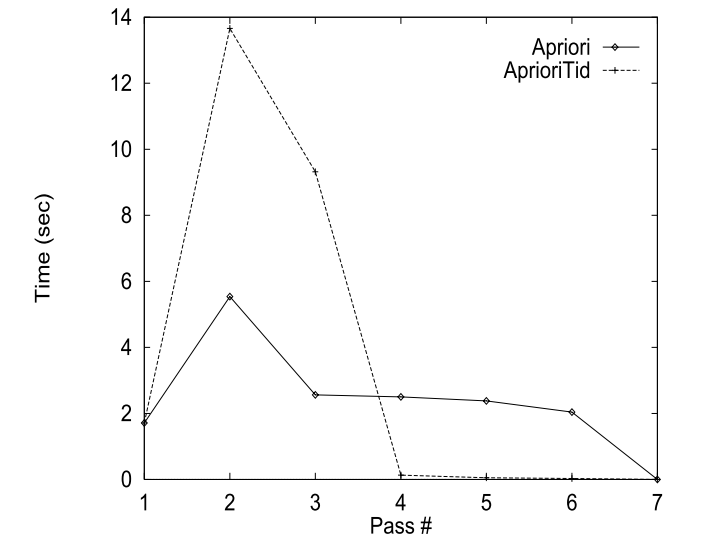
\includegraphics[width=0.7\linewidth]{./images/aprioriVsAprioriTDI}
\caption[Apriori vs AprioriTID]{Vergleich zwischen Apriori und AprioriTID anhand der Dauer pro Durchlauf. Parameter:  Durchschnittliche Größe der Transaktionen = 10, Durchschnittliche Größe der maximalen Kandidatenmenge = 4, Anzahl der Transaktionen = 100.000, minsup = 0.75 \%. \parencite[Quelle:][3.6 Algorithm AprioriHybrid - Figure 6]{IBM}}
\label{fig:aprioriVsAprioriTDI}
\end{figure}


\section{AprioriHybrid}
Das Ziel des AprioriHybrid besteht darin die im letzten Abschnitt (s. \nameref{subsec:vergleichBasicVsTid}) vorgestellten Vorzüge  des Apriori und des AprioriTID zu verbinden (s. Abb.: \ref{fig:hybrid} - \nameref{fig:hybrid}). 
Dieser Hybride Algorithmus verwendet während der Initialisierungsphase den Apriori. 
Dabei wird bei jedem Durchgang geprüft, ob die Größe von $\bar{C}_k \leq$ der Größe des Arbeitsspeichers ist.
Wenn dies der Fall ist wird von Apriori zu AprioriTID gewechselt.
An dieser Stelle ist anzumerken, dass der Wechsel zu AprioriTID mit Kosten verbunden ist. 
Die Entscheidung zum Wechsel wird jeweils am Ende des Durchganges $k$ getroffen. 
Daraufhin wird der Durchgang $k+1$ dafür verwendet, um den AprioriTID zu initialisieren (s. \nameref{aprioriTid}) der schlussendlich erst im Durchgang $k+2$ mit seiner vollen Leistung arbeiten kann \parencite[s.][3.6 Algorithm AprioriHybrid]{IBM}.

\begin{figure}[h]
\centering
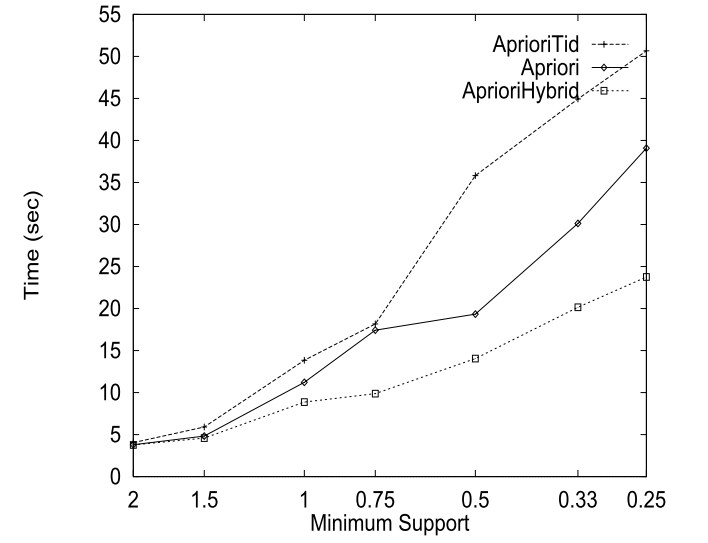
\includegraphics[width=0.7\linewidth]{./images/hybrid}
\caption[Apriori vs AprioriTID vs AprioriHybrid]{Vergleich zwischen Apriori, AprioriTID und AprioriHybrid anhand der Dauer. Parameter: Durchschnittliche Größe der Transaktionen = 10, Durchschnittliche Größe der maximalen Kandidatenmenge = 4, Anzahl der Transaktionen = 100.000 \parencite[Quelle:][3.6 Algorithm AprioriHybrid - Figure 7]{IBM}}
\label{fig:hybrid}
\end{figure}






\appendix

\nocite{*}
\printbibliography
% Acronyms
\subfile{./acronyms.tex}
\include{tex/chapter/appendix}
\end{document}